% !TeX spellcheck = en_GB
\def\ChapterTitle{Modelling and Analysis of Collaborative Node Kinematic Behaviours in Underwater Acoustic MANETs}

\ifx\ifthesis\undefined
\documentclass[a4paper, 11pt]{article}

% % Special Includes stolen from Thesis.cls
\usepackage{booktabs}
\usepackage{hyperref}
\usepackage{graphicx}
\usepackage{epstopdf}
\usepackage{subcaption}
\usepackage{rotating}
\usepackage{listings}
\usepackage{lstpatch}
\renewcommand{\arraystretch}{1.3}

% % % % % % % % % % % % % % % %

% PACKAGES
\usepackage[square, numbers, comma, sort&compress]{natbib}  % Use the "Natbib" style for the references in the Bibliography
\usepackage{verbatim,listings}  % Needed for the "comment" environment to make LaTeX comments
\usepackage{array}  % Needed for the "comment" environment to make LaTeX comments
\usepackage{vector}  % Allows "\bvec{}" and "\buvec{}" for "blackboard" style bold vectors in maths
\usepackage{amsmath,amsfonts,amsthm,color,psfrag,epsf, tabularx, multirow, longtable}
\usepackage{snapshot, todonotes}
% \usepackage{pstricks}
\usepackage{enumerate}
%\usepackage[lined,algonl,boxed]{algorithm2e}
\usepackage[ruled,linesnumbered,vlined]{algorithm2e}
\usepackage{float}
\usepackage{epigraph} % epigraph
\usepackage{tikz}
\usetikzlibrary{shapes.geometric, arrows}

\usepackage{setspace}
\doublespacing
% or:
%\onehalfspacing

% SETUP
\hypersetup{urlcolor=blue, colorlinks=false}  % Colours hyperlinks in blue, but this can be distracting if there are many links. 
\DeclareGraphicsExtensions{.pdf,.jpeg,.png}
\graphicspath{{../Figures/}{../../../Dropbox/Thesis_Figures/}}  % Location of the graphics files (set up for graphics to be in PDF format)

% NOTE THERES A FUCKUP IN TEX4HT http://tug.org/pipermail/tex4ht/2014q2/000944.html
% NEED TO MANUALLY CHANGE \def\pgfsys@svg@newline{{?nl}}
\ifdefined\HCode
\usepackage[compatibility=false]{caption}
\def\pgfsysdriver{pgfsys-tex4ht.def}
\else
\usepackage[]{caption}
\fi

% \SpecialCoor
\def\subsum{\mathit{\Sigma}}

%opening
\title{\ChapterTitle}
\author{Andrew Bolster}

\begin{document}

\maketitle

\else
\chapter{\ChapterTitle}
\label{Chapter\thechapter}
\lhead{Chapter \thechapter. \emph{\nameref{Chapter\thechapter}}} % Write in your own chapter title to set the page header
\fi




\section{Introduction}\label{sec:introduction}
% no \IEEEPARstart
% You must have at least 2 lines in the paragraph with the drop letter
% (should never be an issue)

As mobile ad-hoc networks (MANETs) grow beyond the terrestrial arena, their operation and the protocols designed around them must be reviewed to assess their suitability to different communications environments to ensure their continued security, reliability, and performance.

One area of application is the underwater marine environment, where extreme challenges to communications present themselves (propagation delays, frequency dependent attenuation, fast and slow fading, refractive multi-path distortion, etc.).
In addition to the communications challenges, other considerations such as command and control isolation, as well as power and locomotive limitations, drive towards the use of teams of smaller and cheaper autonomous underwater vehicles (AUVs). 
These increasingly decentralised applications present unique threats against trust management \cite{Caiti2011}.
In underwater environments, communications is both sparse and noisy.
Therefore the observations about the communications processes that are used to generate the trust metrics, occur much less frequently, with much greater error (noise) and delay than is experienced in terrestrial RF MANETS.
As such, the use of trust methods developed in the terrestrial MANET space must be re-appraised for application within the underwater context \cite{Pavan2015}.

Trust Management Frameworks (TMFs) provide information to assist the estimation of future states and actions of nodes within networks.
This information is used to optimize the performance of a network against malicious, selfish, or defective misbehaviour by one or more nodes.
Previous research has established the advantages of implementing TMFs in 802.11 based MANETs, particularly in terms of preventing selfish operation in collaborative systems \cite{Li2007}, and maintaining throughput in the presence of malicious actors \cite{Buchegger2002}

Most current TMFs use a single type of observed action to derive trust values, typically successfully delivered or forwarded packets. 
These observations then inform future decisions of individual nodes, for example, route selection \cite{Li2008}.

Recent work has demonstrated the use of a number of metrics to form a ``vector'' of trust.
The Multi-parameter Trust Framework for MANETs (MTFM) \cite{Guo11}, uses a range of communications metrics beyond packet delivery/loss rate (PLR) to assess trust.
This vectorized trust also allows a system to detect and identify the tactics being used to undermine or subvert trust.
To date this work has been limited to terrestrial, RF based networks. 

The paper is laid out as follows.
In Section \ref{sec:trustandtmfs} we discuss Trust and TMFs, defining our terminology and reviewing the justifications for the use and development of TMFs for marine acoustic networks (MANs)
In Section \ref{sec:marineacousticnetworks} we review selected features of the underwater communications channel, highlighting particular challenges against terrestrial equivalents.
In Section \ref{sec:initialsystemcharacterization} we establish an experimental configuration for the marine space, and review the scenarios and results presented in \cite{Guo11}.
In Section \ref{sec:trustresultsanddiscussion} we present our findings in trust establishment and malicious behaviour detection, comparing with other current TMFs (Hermes and OTMF) and analyse the use of this multi-parameter approach to detecting malicious and selfish behaviour in autonomous marine networks.

The contributions of this paper are a study on the comparative operation and performance of TMFs in marine acoustic networks, and a review of metric suitability for TMFs in marine environments, informing future metric selection for experimenters and theorists.
We also show that single metric trust systems are not directly suitable for the marine context in terms of the different threat and cost scenario in that environment.
Finally, we demonstrate a methodology to assess the usefulness of metrics in discriminating against misbehaviours in such constrained, delay-tolerant networks.



\section{Trust and Trust Management Frameworks}\label{sec:trustandtmfs}


\subsection{Trust in Conventional MANETs}\label{sec:trustinmanets}

The distributed and dynamic nature of MANETs mean that it is difficult to maintain a trusted third party (TTP) or evidence based trust system such as Certificate Authorities (CA) or Public Key Infrastructure (PKI).
Distributed trust management frameworks aim to detect, identify, and mitigate the impacts of malicious actors by distributing per-node assessments and opinions to collectively police behaviour.
Various models and algorithms for describing trust and developing trust management in distributed systems, P2P communities or wireless networks have been considered.
\emph{Hermes Trust Establishment Framework} takes a Bayesian Beta function to model per-link Packet Loss Rate (PLR) over time, combining ``Trust'' and ``Confidence of Assessment'' into a single value \cite{Zouridaki2005}.
\emph{Objective Trust Management Framework} (OTMF) builds upon Hermes and distributes node observations across the network \cite{Li2008}, however does not appropriately combat multi-node-collusion in the network \cite{Cho2011}.
\emph{Trust-based Secure Routing} demonstrated an extension to Dynamic Source Routing (DSR), incorporating a Hidden Markov Model of sub-networks, reducing the efficacy of Byzantine attacks such as black-hole routing  \cite{Moe2008a}.
\emph{CONFIDANT} presented an approach using a probabilistic estimation of PLR, similar to OTMF, also introducing a topology aware weighting scheme and also weighting trust assessments based on historical experience of the reporter \cite{Buchegger2002}.
\emph{Fuzzy Trust-Based Filtering} uses Fuzzy Inference to adapt to malicious recommenders using conditional similarity to classify performance with overlapping fuzzy set membership, filtering assessments across a network \cite{Luo2008}. 

These TMFs can be generalised as single-value estimation based on a binary input state (success or failure of packet delivery) and generating a probabilistic estimation of the future states of that input. 

These single metric TMFs provide malicious actors with a significant advantage if their activity does not impact that metric.
In the case where the attacker can subvert the TMF, the metric under assessment by that TMF does not cover the threat mounted by the attacker.
This causes a significant negative effect on the efficiency of the network, as the TMF is assumed to have reduced the possible set of attacks when it has actually made it more advantageous to attack a different part of the networks operation.
An example of such a situation would be in a TMF focused on PLR where an attacker selectively delays packets going through it, reducing overall throughput but not dropping any packets.
Such behaviour would not be detected by the TMF.

For the purposes of this work, we select Hermes trust establishment and OTMF as indicative single-metric TMFs to compare against MTFM, as Hermes captures the core operation of a pure single metric assessment methodology and OTMF provides a comparison that combines assessments from across nodes to develop trust opinions.


\subsection{Trust in Marine Networks}\label{sec:trust_in_marine}

With demand for smaller, more decentralised marine survey and monitoring systems, and a drive towards lower per-unit cost, pressures on battery capacity, locomotive power efficiency, data processing and storage are increasing.
These pressures simultaneously present opportunities and incentives for malicious or selfish actors to appear to cooperate while not reciprocating, in order to conserve power for instance.

Within UANs observable metrics include significant noise and may occur at irregular and sparse intervals.
Conventional approaches such as probabilistic estimation do not produce trust values that reflect the underlying reality and context of the metrics available, as they require a-priori assumption that the trust value under exploration has an expected distribution, that distribution is mono-modal, and the input metrics are binary.
In scenarios with variable, sparse, noisy metrics, estimating the distribution is difficult to accomplish a-priori.

\subsection{Single Metric Trust Frameworks}

The Hermes trust establishment framework \cite{Zouridaki2005} uses Bayesian reasoning to generate a posterior distribution function of ``belief'', or trust, given a sequence of observations of that behaviour, $p(B|O)$\eqref{eq:otmf_pbo}.

\begin{equation}
	p(B|O)  = \frac{p(O|B) \times p(B)}{\rho}
	\label{eq:otmf_pbo}
\end{equation}

Where $p(B)$ is the prior probability density function for the expected normal behaviour, and $\rho$ is a normalising factor.
Due to it's flexibility and simplicity, Hermes assumes that $p(B)$ is a Beta function, and therefore the evaluation of this trust assessment is based around the expectation value of the distribution \eqref{eq:otmf_t}  where $\alpha$ and $\beta$ represent the number of successful and unsuccessful interactions respectively for a particular node $i$.

A secondary measurement of the confidence factor of the trust assessment $t$ is generated as \eqref{eq:otmf_c} and these measurements are combined to form a ``trustworthiness'' value $T$ \eqref{eq:otmf_trust}.

\begin{align}
	t_i &\to E\lbrack\text{beta}(p|\alpha,\beta)\rbrack = \frac{\alpha_i}{\alpha_i+\beta_i} \label{eq:otmf_t}\\[5pt]
	c_i &= 1 - \sqrt{\frac{12\alpha_i\beta_i}{(\alpha_i+\beta_i)^2(\alpha_i+\beta_i+1)}} \label{eq:otmf_c}\\[5pt]
	T_i &= 1 - \frac{\sqrt{\frac{(t_i-1)^2}{x^2} + \frac{(c_i-1)^2}{y^2}}}{\sqrt{\frac{1}{x^2}+\frac{1}{y^2}}} \label{eq:otmf_trust}
\end{align}

In \eqref{eq:otmf_trust}, $x$ and $y$ are constants, used weight the two-dimensional polar mapping of trust and confidence assessments ($t_i,c_i$), and from \cite{Zouridaki2005}, are taken as $x=\sqrt{2},y=\sqrt{9}$.

Upon this per-node assessment methodology, OTMF overlays an observation distribution protocol so as to make the measurements $\alpha_i$ and $\beta_i$ representative of the direct and 1-hop networks observations of the target node $i$, as well as expiring old observations from assessment and eliminating observations from ``untrustworthy'' nodes.


\subsection{Multi-Metric Trust Frameworks}\label{sec:multimetrictrust}

Given the potential incentives to a selfish attacker and potential threats to trust and fairness in sparse, noisy, and constrained environments, single metric trusts discussed above do not suitably cover the exposed threat surface. 
This indicates that a multi-metric approach may be more appropriate to capture and monitor the realities of an environment such as those experienced by UANs.

Grey Theory performs cohort based normalization of metrics at runtime, providing a ``grade'' of trust compared to other observed nodes in that interval, while maintaining the ability to reduce trust values down to a stable assessment range for decision support without requiring every environment entered into to be characterised.
This presents a stark difference between the Grey and Probabilistic approaches.
Grey assessments are relative in both fairly and unfairly operating networks.
All nodes will receive mid-range trust assessments if there are no malicious actors as there is nothing ``bad'' to compare against, and variations in assessment will be primarily driven by topological and environmental factors.
Guo et al. \cite{Guo11} demonstrated the ability of grey relational analysis (GRA) \cite{Zuo1995} to normalise and combine disparate traits of a communications link such as instantaneous throughput, received signal strength, etc. into a grey relational coefficient (GRC), or a ``trust vector'' in this instance.

The grey relational vector is given as
%
\begin{align}
	\label{eq:grc}
	\theta_{k,j}^t = \frac{\min_k|a_{k,j}^t - g_j^t| + \rho \max_k|a_{k,j}^t-g_j^t|}{|a_{k,j}^t-g_j^t| + \rho \max_k|a_{k,j}^t-g_j^t|} \\
	\phi_{k,j}^t = \frac{\min_k|a_{k,j}^t - b_j^t| + \rho \max_k|a_{k,j}^t-b_j^t|}{|a_{k,j}^t-b_j^t| + \rho \max_k|a_{k,j}^t-b_j^t|} \notag 
\end{align}
%
where $a_{k,j}^t$ is the value of an observed metric $x_j$ for a given node $k$ at time $t$, $\rho$ is a distinguishing coefficient set to $0.5$, $g$ and $b$ are respectively the ``good'' and ``bad'' reference metric sequences from $\{a_{k,j}^t k=1,2\dots K\}$, i.e. $g_j=\max_k({a_{k,j}^t})$,  $b_j=\min_k({a_{k,j}^t})$ (where each metric is selected to be monotonically positive for trust assessment, e.g. higher throughput is presumed to be always better). 

Weighting can be applied before generating a scalar value \eqref{eq:metric_weighting} allowing the detection and classification of misbehaviours.

%
\begin{equation}
	\label{eq:metric_weighting}
	[\theta_k^t, \phi_k^t] = \left[\sum_{j=0}^M h_j \theta_{k,j}^t,\sum_{j=0}^M h_j \phi_{k,j}^t \right]
\end{equation}
%
Where $H=[h_0\dots h_M]$ is a metric weighting vector such that $\sum h_j = 1$, and in unweighted case, $H=[\frac{1}{M},\frac{1}{M}\dots\frac{1}{M}]$.
$\theta$ and $\phi$ are then scaled to $[0,1]$ using the mapping $y = 1.5 x - 0.5$.
To minimise the uncertainties of belonging to either best ($g$) or worst ($b$) sequences in \eqref{eq:grc} the $[\theta,\phi]$ values are reduced into a scalar trust value by $T_k^t = ({1+{(\phi_k^t)^2}/{(\theta_k^t)^2}})^{-1}$ \cite{Hong2010}.
MTFM combines this GRA with a topology-aware weighting scheme \eqref{eq:networkeffects} and a fuzzy whitenization model \eqref{eq:whitenization}. 

There are three classes of topological trust relationship used; Direct, Recommendation, and Indirect.
Where an observing node $n_i$ assesses the trust of another target node, $n_j$; the Direct relationship is $n_i$'s own observations $n_j$'s behaviour.
In the Recommendation case, a node $n_k$ which shares Direct relationships with both $n_i$ and $n_j$, gives its assessment of $n_j$ to $n_i$.
In the Indirect case, similar to the Recommendation case, the recommender $n_k$ does not have a direct link with the observer $n_i$ but $n_k$ has a Direct link with the target node, $n_j$.
These relationships give node sets, $N_R$ and $N_I$ containing the nodes that have recommendation or indirect, relationships to the observing node respectively.
%
\begin{align}
	\label{eq:networkeffects}
	T_{i,j}^{MTFM}=&\frac{1}{2} \cdot \max_s\{f_s(T_{i,j})\} T_{i,j}\\ \notag
	+&\frac{1}{2} \frac{2|N_R| }{2|N_R| + |N_I|}\sum_{n \in N_R} \max_s\{f_s(T_{i,n})\} T_{i,n}\\ \notag
	+&\frac{1}{2} \frac{|N_I| }{2|N_R| + |N_I|}\sum_{n \in N_I} \max_s\{f_s(T_{i,n})\} T_{i,n} 
\end{align}

Where $T_{i,n}$ is the subjective trust assessment of $n_i$ by $n_n$, and $f_s = [ f_1,f_2, f_3]$ given as:

\begin{align}
	\label{eq:whitenization}
	f_1(x)&= -x+1\notag\\
	f_2(x)&= 
	\begin{cases}
		2x & \text{if }x\leq 0.5\\
		-2x+2 & \text{if }x>0.5
	\end{cases}\\
	f_3(x)&= x\notag
\end{align}
%
In the case of the terrestrial communications network used in \cite{Guo11}, the observed metric set $X = {x_1,\dots,x_M}$ representing the measurements taken by each node of its neighbours at least interval, is defined as $X=[$packet loss rate, signal strength, data rate, delay, throughput$]$.

Guo et al. demonstrated that when compared against OTMF and Hermes trust assessment, MTFM provided increased variation in trust assessment over time, providing more information about the nodes' behaviours than packet delivery probability alone can.

By weighting the metrics used in MTFM it was shown that the trust assessments could be used to identify the style of misbehaviour being performed within the network, and by whom.
We present a corollary method to investigate and apply this work to the Marine MANET field.


\section{Marine Acoustic Communications}\label{sec:marineacousticnetworks}

The key challenges of underwater acoustic communications are centred around the impact of slow and differential propagation of energy (RF, Optical, Acoustic) through water, and its interfaces with the seabed / air.
The resultant challenges include; long propagation delays, significant inter-symbol interference and Doppler spreading, fast and slow fading due to environmental effects (aquatic flora/fauna, surface weather), carrier-frequency dependent signal attenuation, multi-path caused by reflective medium interfaces, variations in propagation speed due to depth dependant effects (salinity, temperature, and pressure), and subsequent refractive spreading and lensing due to that same propagation variation \cite{Partan2006}.

The attenuation that occurs in an underwater acoustic channel over a distance $d$ for a signal about frequency $f$ in linear power is given as $A_{\text{aco}}(d,f) = A_0d^ka(f)^d$ and in $dB$ form as;
%
\begin{equation}
	\label{eq:acoattenuationdb}
	10 \log A_{\text{aco}}(d,f)/A_0 = k \cdot 10 \log d + d \cdot 10 \log a(f)
\end{equation}
%
where $A_0$ is a normalising constant, $k$ is a spreading factor (commonly taken as 1.5  \cite{Stojanovic2007}), and $a(f)$ is the absorption coefficient, approximated using Thorp's formula \cite{Stefanov2011}
%
\begin{equation}
	\label{eq:thorp}
	10 \log a(f) = \frac{0.11 \cdot f^2}{1+f^2} + \frac{44\cdot f^2}{4100+f^2}+ 2.75\times10^{-4} f^2 + 0.003
\end{equation}
%
Refractive lensing and the multi-path nature of the medium result in line of sight propagation being extremely unreliable for estimating distances to targets.
The first arriving acoustic signal has as the very least curved in the medium, and commonly has reflected off the surface/seabed before arriving at a receiver, creating secondary paths that are sometimes many times longer than the first arrival path, generating symbol spreading over orders of seconds depending on the ranges and depths involved.
Forward Error Correction coding is used on such channels to minimise packet losses.

Comparing $A_{aco}(d,f)$ with the RF Free-Space Path Loss model $(A_{\text{RF}}(d,f) \approx \left( \frac{4\pi d f}{c} \right)^2)$, the impact of range on signal power is exponential underwater, rather than quadratic in terrestrial RF ($A_{\text{aco}} \propto f^{2d}$ vs $A_{\text{RF}} \propto (df)^2$). 
While both frequency dependant factors are quadratic, approximating the factors in \eqref{eq:thorp}, $f\propto A_{\text{aco}}$ is at least 4 orders of magnitude higher than $f\propto A_{\text{RF}}$



\section{System Model Characterization}\label{sec:initialsystemcharacterization}


\subsection{Mobility, Topology, and Communications}

We apply two mobility patterns for investigation; all nodes static and all nodes mobile.
The reason for this is that in other mobility combinations, the node targeted for misbehaviour ($n_1$) will already be behaving differently compared to the rest of the network regardless of the misbehaviour.

The six nodes are initially arranged as per Fig.~\ref{fig:s1_layout} with each node on average 100m from each other as per \cite{Guo11}.
The use of six nodes and the particular layout enables the investigation of the three trust relationships based on minimum path topologies, such that the node generating the trust assessments, $n_0$ has Direct, Recommendation, and Indirect trust assessments of $n_1$ available to it from itself, $[n_2,n_3]$, and $[n_4,n_5]$ respectively. 

Collaborations with NATOs Centre for Maritime Research and Experimentation (CMRE) in La Spezia, and DSTLs Naval Systems Group inform that this is a practical team-size for environmental and defence applications.

%
\begin{figure}[h]
	\centering
	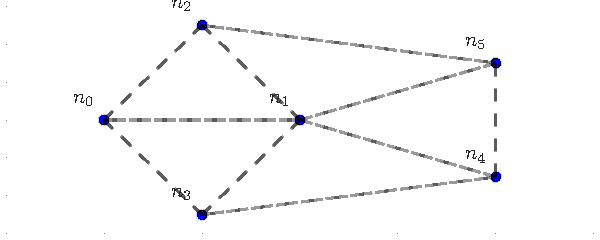
\includegraphics[width=.45\textwidth]{s1_layout}
	\caption{Initial layout with nodes spaced an average of 100m apart}
	\label{fig:s1_layout}
\end{figure}
%

\subsection{Simulation Background}

Simulations were conducted using a Python based simulation framework, SimPy \cite{Mueller2003SimPy}, with a network stack built upon AUVNetSim \cite{Miquel2008}, with transmission parameters (Table \ref{tab:sysconstraints}) taken from and validated against \cite{Stojanovic2007} and \cite{Stefanov2011}.

Given the differences in delay and propagation between RF and marine networks, it would not be expected that the same application rates (e.g. packet emission rates or throughput) and node separations are equally stable in this environment.
Therefore, we first characterise a zone of performance within which the network have stable operation.
%
\begin{table}[h]
	\caption{Comparison of system model constraints as applied between Terrestrial and Marine communications} \label{tab:sysconstraints}
	\begin{center}
		\setlength{\tabcolsep}{8pt}
		\begin{tabular}{lccc}
			\toprule
			Parameter & Unit & Terrestrial & Marine \\
			\midrule
			Simulated Duration & $s$ & 300 & 18000\\
			Trust Sampling Period & $s$ & 1 & 600 \\
			Simulated Area & $km^2$ & 0.7 & 0.7-4 \\
			Transmission Range & $km$ & 0.25 & 1.5 \\
			Physical Layer & & RF(802.11) & Acoustic\\
			Propagation Speed& $m/s$ & $3\times10^8$ & 1490\\
			Center Frequency& $Hz$ & $2.6\times10^9$ & $2 \times 10^4$ \\
			Bandwidth& $Hz$ & $22\times10^6$ & $1\times10^4$\\
			MAC Type & & CSMA/DCF & CSMA/CA\\
			Routing Protocol & & DSDV & FBR \\
			Max Speed & $ms^{-1}$ & 5 & 1.5 \\
			Max Data Rate & $bps$ & $5\times10^6$ & $\approx 240$ \\
			Packet Size & bits & 4096 &  9600 \\
			Single Transmission Duration & $s$ & 10 & 32 \\
			Single Transmission Size & bits & $10^7$ & $9600$ \\
			\bottomrule
		\end{tabular}
		\setlength{\tabcolsep}{6pt}
	\end{center}
\end{table}
%


\subsection{Scaling Considerations between Terrestrial and Underwater Environments}

We establish an appropriate safe operating zone for marine communications by looking at the communications rate and physical distribution factors across the two selected mobility scenarios.
From Table~\ref{tab:sysconstraints}, the operating transmission range of this model of acoustic communications is $\approx 6$ times further than that of 802.11, indicating that a suitable operating environment will have an area $\approx \sqrt{6}$ times the area of the 802.11 case.
However, it was recognised in Section~\ref{sec:marineacousticnetworks} that underwater, the relationship between attenuation and distance is exponential, so this would represent an upper bound of performance, where nodes are approximately 400m apart. 

Exploratory simulations were run to further constrain this bound.
As the separation is increased, the emission rate at which the network becomes saturated decreases, reducing overall throughput. 
This throughput degradation is tightly coupled with the mobility, as increasing mobility leads to increasing delays as routes are constantly broken, re-advertised and re-established. 
For instance, where all nodes are static, we do not see significant drops in saturation rates until node separation approaches 800m, nearly double the initial estimate. 
When all nodes are randomly walking the saturation point collapses from 0.025pps at 300m to 0.015pps at 400m.
Our results indicate that the best area to continue operating in for a range of node separations is at 0.015pps, and that a reasonable position scaling is from 100m to 300m, beyond which communication becomes increasingly unstable, especially in terms of end-to-end delay.
These results are similar to work performed in \cite{Miquel2008}, and are expected in such a sparse, noisy, and contentious environment. 


\subsection{Selected Misbehaviours}


We are primarily concerned with the direct trust relationship between $n_0$ and $n_1$, i.e. $n_0$'s assessment of the trustworthiness of $n_1$, or $T_{1,0}$.

Guo et al. introduce a range of misbehaviours, including modification of the packet loss rate of routing nodes and limiting throughput on a per-link basis as well as a selection of combined misbehaviours. 
Given that the established links are already heavily constrained, such attacks would severely impact the general performance of the network beyond the scope of simple selfishness.
These direct malicious behaviours effectively trigger saturation collapses in operating regions of the network that should be stable.

Therefore, we apply two more subtle misbehaviours to investigate; 
\begin{enumerate}
	\item Malicious Power Control (MPC), where $n_1$ increases its transmit and forwarding power by 20\% for all nodes \emph{except} communications from $n_0$ in order to make $n_0$ appear to be selfishly conserving energy to the rest of the team, while $n_1$ itself appears to be performing very well.
	\item Selfish Target Selection (STS), where $n_1$ preferentially communicates, forwards and advertises to nodes that are physically close to it in effort to reduce its own power consumption.
\end{enumerate}


\section{Simulation Results and Discussion}\label{sec:trustresultsanddiscussion}

Having established a safe operating range for comparison at 300m average separation and an emission rate of 0.015pps, we perform each of the three selected behaviours (Fair, MPC, STS) in both the static and mobile scenarios. 
We select a trust assessment period of 10 mins for a 5 hour mission to scale in comparison to relative bitrates experienced (1Mbps vs $\approx15$bps).

The six metrics used for grey assessment are; transmitted and received throughput and power, delay, and packet loss rate (PLR) as calculated by aborted and unacknowledged, transmissions.
Compared to \cite{Guo11}, this metric set lacks a data rate quantity as the network is not dynamically adjusting bandwidth.
In context of GRC generation \eqref{eq:grc}, the best sequence $g$ was selected using the lowest PLR, delay, and powers, and the highest throughputs, and the worst sequence, $b$ the inverse of these metrics, reflecting the observations made in Section~\ref{sec:trust_in_marine}.

The particular factors under discussion are the relative performance of MTFM against OTMF and Beta with respect to statistical stability across mobilities and in responsiveness to changing network behaviour. 
We establish a similar result set by initially tracking the resultant trust values established by MTFM in the pair of mobility scenarios, shown in Fig.~\ref{fig:trust_mobility}.
We are also concerned with the opinions of $n_1$ provided to $n_0$ by other nodes, where $[T_{1,2},T_{1,3}]$ and $[T_{1,4},T_{1,5}]$ denote the sets of recommendation and indirect trust assessment respectively.

We also include aggregate assessments; $T_{1,\text{Avg}}$, the unweighted mean of direct trust assessments of $n_1$ from all nodes and $T_{1,\text{MTFM}}$, the final MTFM trust assessment value based on both network topology and whitenization from \eqref{eq:whitenization}.

The variability in assessment is coupled to mobility; in the static case (Fig.~\ref{fig:trust_static}), we see that the nodes exhibit relatively consistent distributions.
In the full mobility case, shown in Fig.~\ref{fig:trust_all_mobile}, this subjective variability is greatly increased. 
As the topology is highly dynamic, delays due to re-establishing routes can be very large, perturbing the trust value.
The $T_{1,\text{MTFM}}$ displays a significantly reduced variation than those of the individual subjective observations in all cases, even when compared to the unweighted average, $T_{1,\text{Avg}}$.
This demonstrates $T_{MTFM}$'s value as an aggregating trust assessment in such sparse and noisy environments.
Further, in Fig.~\ref{fig:trust_all_mobile_mal} we observe a much higher variability in assessment in $T_0$, correctly indicating that there is something wrong with the relationship between $n_0$ and $n_1$.

\begin{figure}[h]
	\centering
	\begin{subfigure}{0.5\textwidth}
	\caption{Fair Static}
	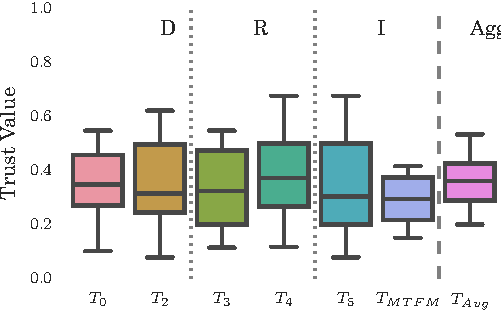
\includegraphics[width=\linewidth]{trust_bella_static_fair} 
	\label{fig:trust_static}
	\end{subfigure}%
	\begin{subfigure}{0.5\textwidth}
	\caption{Fair Mobile}
	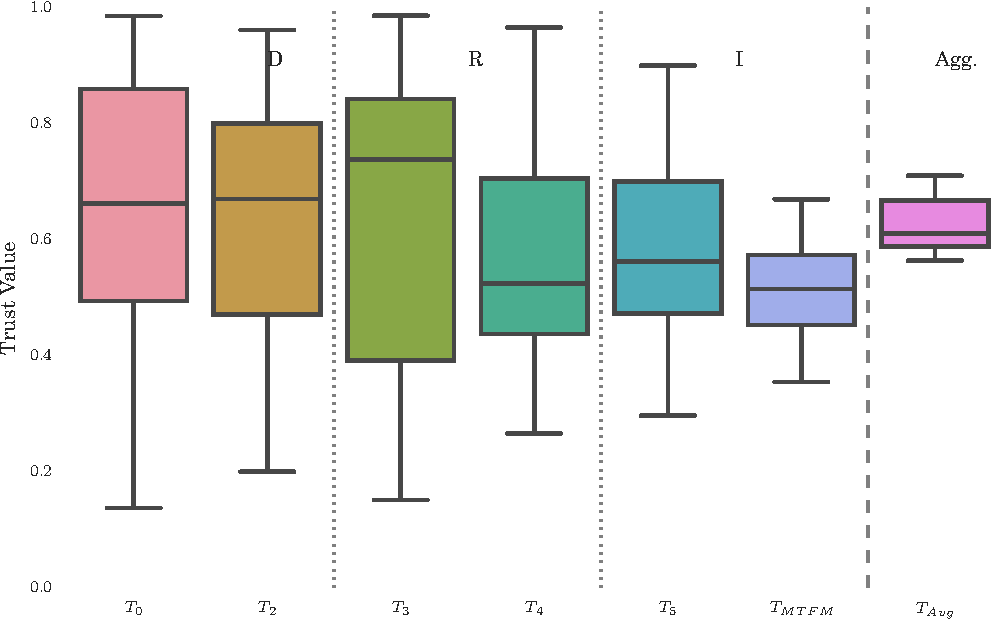
\includegraphics[width=\linewidth]{trust_bella_all_mobile_fair}  
	\label{fig:trust_all_mobile}
	\end{subfigure}%
	
	\begin{subfigure}{0.5\textwidth}
	\caption{Malicious Static}
	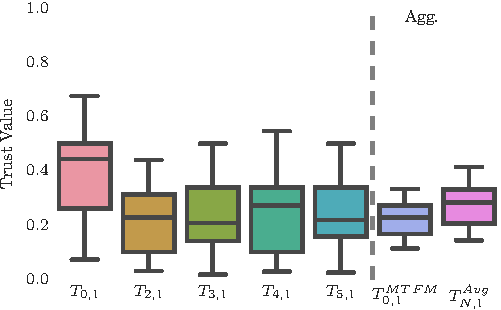
\includegraphics[width=\linewidth]{trust_bella_static_malicious} 
	\label{fig:trust_static_mal}
	\end{subfigure}%
	\begin{subfigure}{0.5\textwidth}
	\caption{Malicious Mobile}
	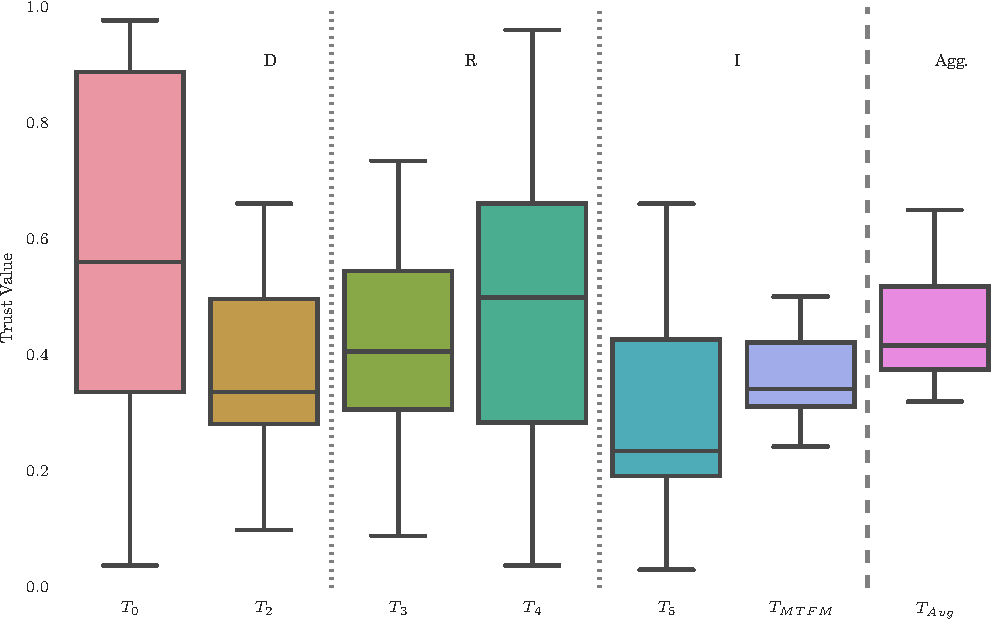
\includegraphics[width=\linewidth]{trust_bella_all_mobile_malicious}  
	\label{fig:trust_all_mobile_mal}
	\end{subfigure}%
	
	\begin{subfigure}{0.5\textwidth}
	\caption{Selfish Static}
	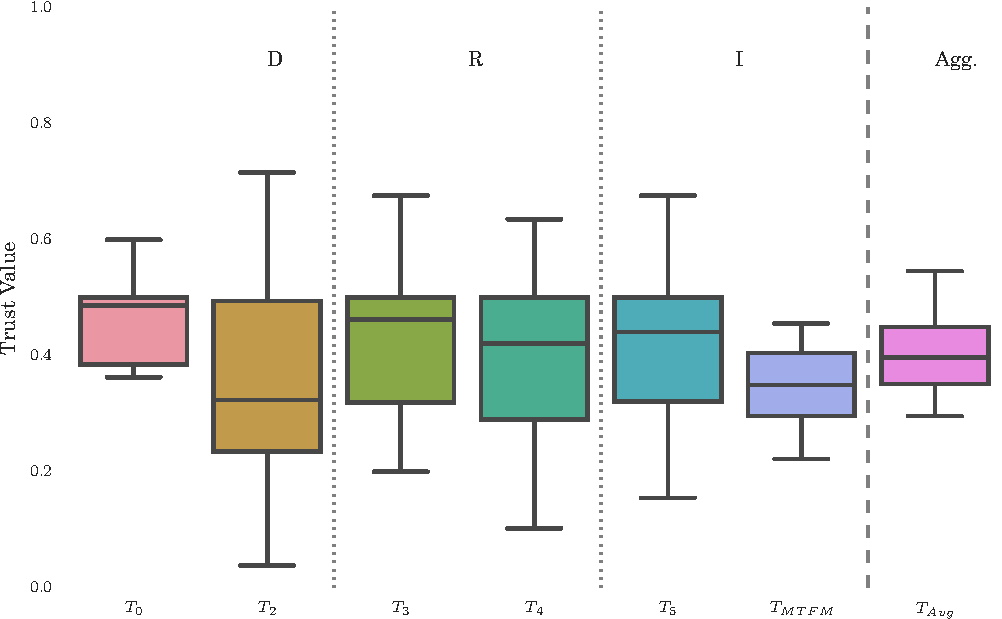
\includegraphics[width=\linewidth]{trust_bella_static_selfish}
	\label{fig:trust_static_sel}
	\end{subfigure}%
	\begin{subfigure}{0.5\textwidth}
	\caption{Selfish Mobile}
	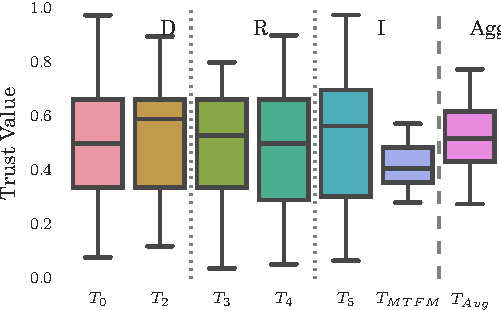
\includegraphics[width=\linewidth]{trust_bella_all_mobile_selfish}  \label{fig:trust_all_mobile_sel}
	\end{subfigure}%

	\caption{MTFM Trust assessments of $n_1$ ($T_{1,X}$), showing Direct, Recommender and Indirect relationships, as well as the Aggregate trust assessments from combining these} 
	\label{fig:trust_mobility}
\end{figure}
%

\subsection{Comparison between MTFM, Hermes and OTFM}
As per \cite{Guo11}, ``fair'' scenarios were also performed with no malicious behaviour, applying OTMF and Hermes assessment as well as MTFM, providing like-for-like comparison of assessment.
For simplicity of presentation, we only consider the fully-mobile scenario, as we are concerned with the establishment of trust in mobile networks

\begin{figure*}[t]
	\begin{subfigure}{0.32\textwidth}	
	\caption{Fair Scenario}
	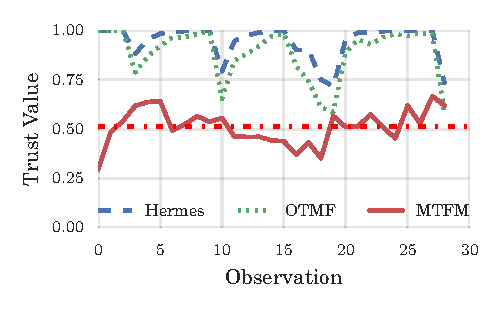
\includegraphics[width=\linewidth]{trust_beta_otmf_fair}
	\label{fig:all_mobile_fair_beta}
	\end{subfigure}
	\begin{subfigure}{0.32\textwidth}
	\caption{Malicious Power Control Scenario}
	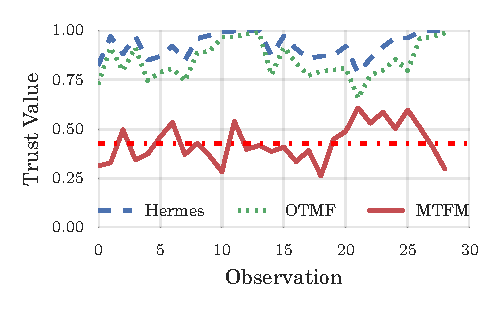
\includegraphics[width=\linewidth]{trust_beta_otmf_malicious} 
	\label{fig:all_mobile_badmouthing_beta}
	\end{subfigure}
	\begin{subfigure}{0.32\textwidth}	
	\caption{Selfish Target Selection Scenario}
	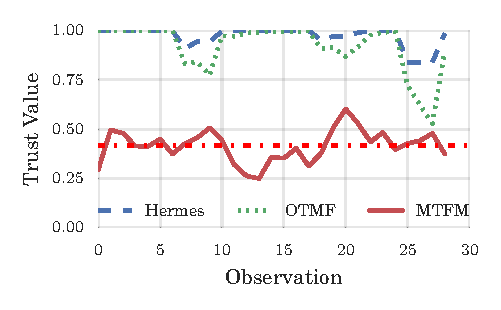
\includegraphics[width=\linewidth]{trust_beta_otmf_selfish} 
	\label{fig:all_mobile_selfish_beta}
	\end{subfigure}
	\caption{$T_{1,0}$ for Hermes, OTMF and MTFM assessment values for fair and malicious behaviours in the fully mobile scenario (mean of MTFM also shown)}
	\label{fig:otmf_beta_comparison}
\end{figure*}
%
The use of Forward Beam Routing and a CSMA/CA MAC scheme from AUVNetSim \cite{Miquel2008} in our simulation mitigates a significant number of packet losses through collision avoidance and contention handling, leading to the situation that the only genuinely lost packets occur when a node moves completely out of range of any other node and time out occurs in route discovery rather than transmission.
As such, confirmed packet losses are relatively rare and in a delaying network like this, it is difficult to set a differentiating time out between packets that are in the network but queued, and packets that are actually ``lost''.

The single metric TMFs used in conventional MANETs require regular and constant input to shape and adjust their evaluations, which for a network with significant and irregular delays such as this, is not practical.
This renders OTMF and Hermes assessment at best uninformative and at worst misleading; consistently providing nodes a high trust assessment as they have very little information to extract trust from. 

Fig.~\ref{fig:otmf_beta_comparison} shows a comparison between the unweighted response of MTFM compared to OTMF and Hermes assessment functions on the same data for the fair, malicious and selfish behaviours respectively.
It is important to note a distinction between the expectations of MTFM compared to other TMFs; MTFM is primarily concerned with the identification of differences in the behaviours of nodes in a network, and is relative rather than absolute.
That is to say that under MTFM, nodes are compared against the worst current performances across metrics of other observed nodes and graded against them, rather than the absolute (objective) approach taken by many TMFs.
In these cases, particularly since the methods of attack were not directly related to PLR, OTMF and Hermes have not registered significant activity in either misbehaviour when compared to the fair scenario.
The difference between the MTFM trust assessments under ``fair'' and ``malicious'' behaviour is lowered by $\approx 10\%$ in both cases, in terms of the mean values returned.
At run time, similar results could be attained by an exponentially weighted moving average filter (EWMA).

On their own, neither OTMF, Hermes, or unbiased MTFM appear to be effective in detecting or identifying malicious behaviour in this environment, in fact OTMF and Hermes don't appear to differentiate between fair and selfish scenarios at all.


\subsection{Metric Weighting}
%

We apply a sequence of vectors that preferentially weight each metric in Eq. \eqref{eq:metric_weighting} to each of the three simulation runs.
For a metric weight vector $H$, where the metric $m_j$ is emphasised as being twice as important as the other metrics, we form an initial weighting vector $H'=[h_i...h_M]$ such that $h_i = 1 \forall i \ne j; h_j=2$. We then scale that vector $H'$ such that $\sum H = 1$ by $H= \frac{H'}{\sum H'}$.
Using this process we can extract and highlight the primary aspects of an attack by comparing against the deviation from the ``fair'' result set. 

\begin{figure}[h]
	\centering
	\begin{subfigure}{0.5\textwidth}
		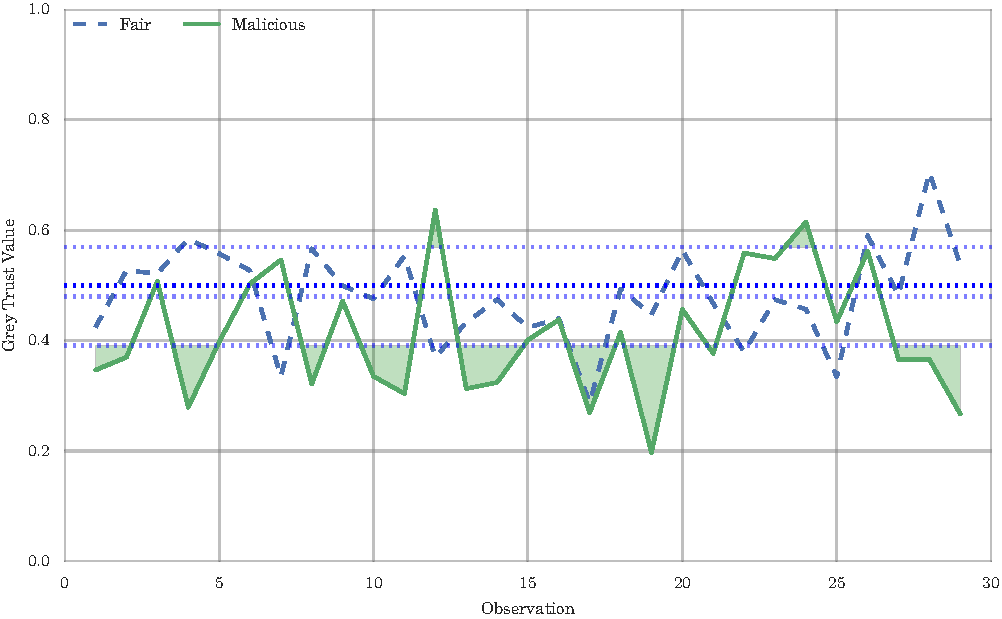
\includegraphics[width=.45\linewidth]{trust_bella_all_mobile_emph_ADelay_BadMouthingPowerControl} \label{fig:all_mobile_badmouthing_delay}
		\caption{Delay Emphasised}
	\end{subfigure}
	\begin{subfigure}{0.5\textwidth}
		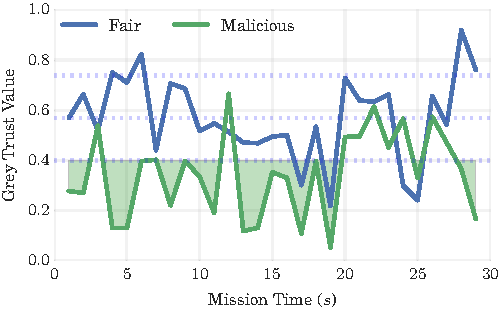
\includegraphics[width=.45\linewidth]{trust_bella_all_mobile_emph_PLR_BadMouthingPowerControl}
		\label{fig:all_mobile_badmouthing_plr}
		\caption{PLR Emphasised}
	\end{subfigure}
	
	\begin{subfigure}{0.5\textwidth}
		\caption{RX Power Emphasised}
		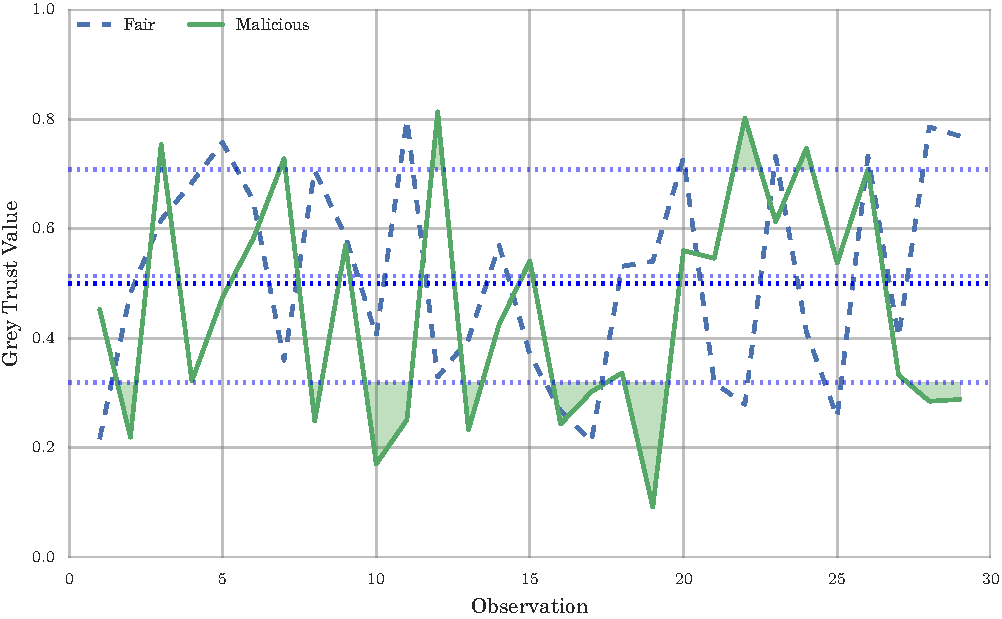
\includegraphics[width=.45\linewidth]{trust_bella_all_mobile_emph_ARXP_BadMouthingPowerControl} 
		\label{fig:all_mobile_badmouthing_rxp}
		\caption{TX Power Emphasised}
	\end{subfigure}	
	\begin{subfigure}{0.5\textwidth}
		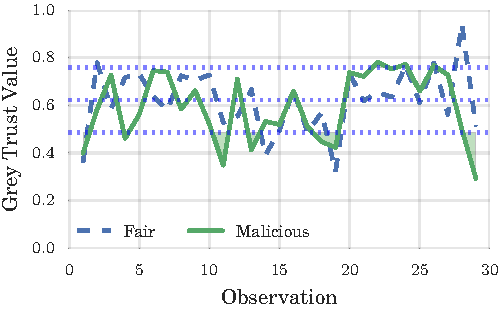
\includegraphics[width=.45\linewidth]{trust_bella_all_mobile_emph_ATXP_BadMouthingPowerControl}
		\label{fig:all_mobile_badmouthing_txp}
	\end{subfigure}
	
	\begin{subfigure}{0.5\textwidth}
		\caption{RX Throughput Emphasised}
		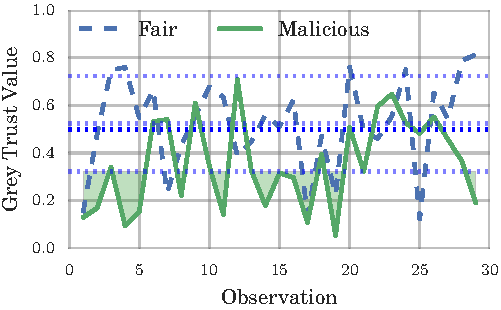
\includegraphics[width=.45\linewidth]{trust_bella_all_mobile_emph_RXThroughput_BadMouthingPowerControl} \label{fig:all_mobile_badmouthing_rxthroughput}
	\end{subfigure}
	\begin{subfigure}{0.5\textwidth}
		\caption{TX Throughput Emphasised}
		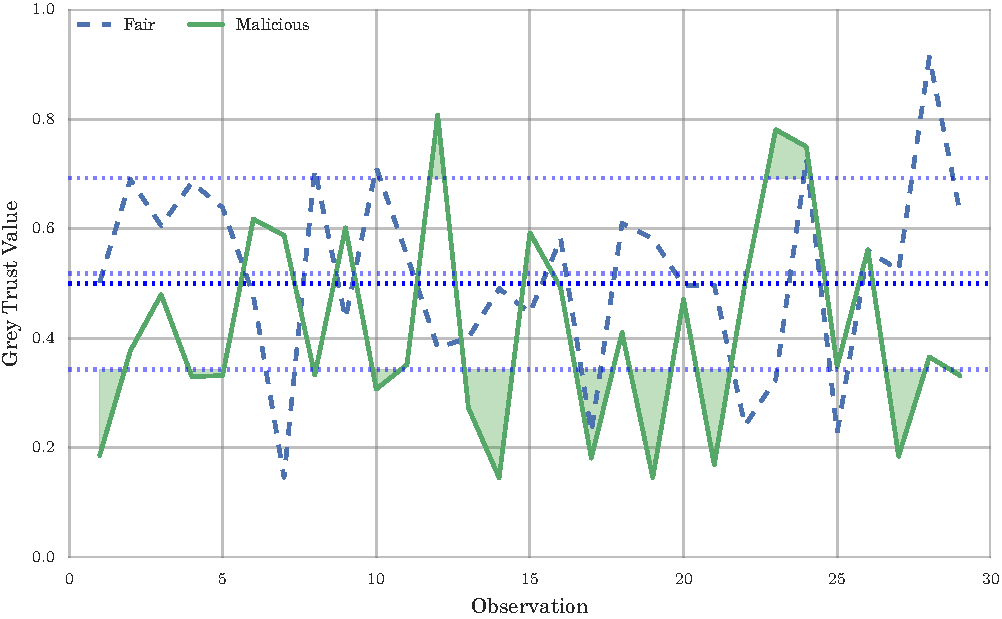
\includegraphics[width=.45\linewidth]{trust_bella_all_mobile_emph_TXThroughput_BadMouthingPowerControl} \label{fig:all_mobile_badmouthing_txthroughput}
	\end{subfigure}
	\caption{$T_{1,MTFM}$ in the All Mobile case for the Malicious Power Control behaviour, including dashed $\pm\sigma$ envelope about the fair scenario}
	\label{fig:all_mobile_badmouthing}
\end{figure}
%
\begin{figure}[h]
	\centering
	\begin{subfigure}{0.45\textwidth}	
	\caption{Delay Emphasised}
	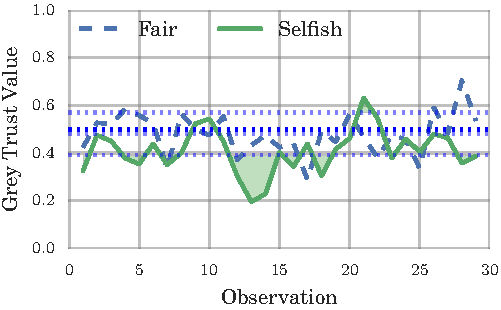
\includegraphics[width=\linewidth]{trust_bella_all_mobile_emph_ADelay_SelfishTargetSelection} 
	\label{fig:all_mobile_selfish_delay}
	\end{subfigure}
	\begin{subfigure}{0.45\textwidth}	
	\caption{PLR Emphasised}
	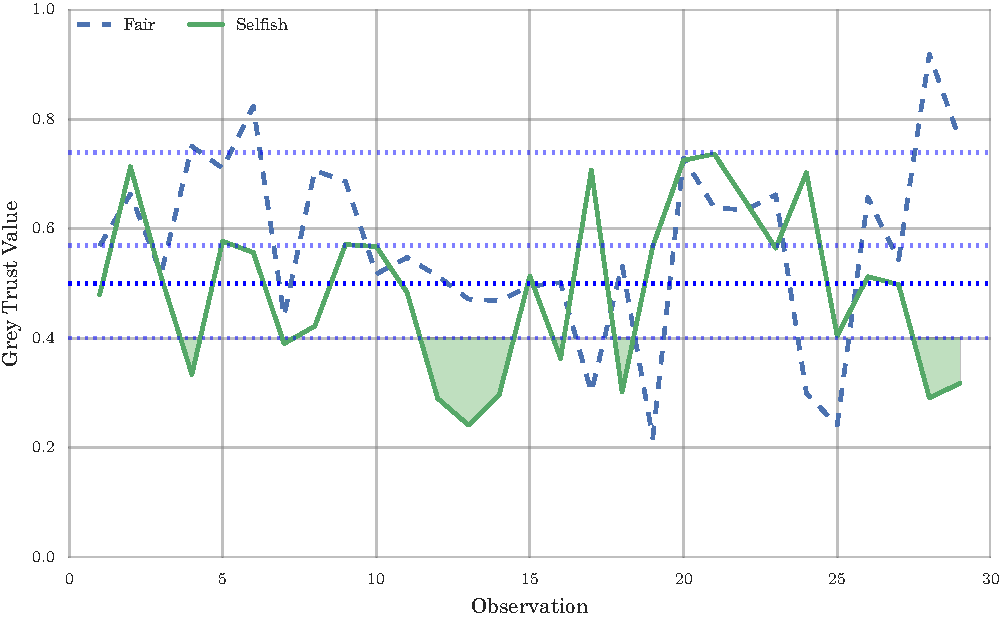
\includegraphics[width=\linewidth]{trust_bella_all_mobile_emph_PLR_SelfishTargetSelection}
	\label{fig:all_mobile_selfish_plr}
	
	\end{subfigure}
	\begin{subfigure}{0.45\textwidth}	
	\caption{RX Power Emphasised}
	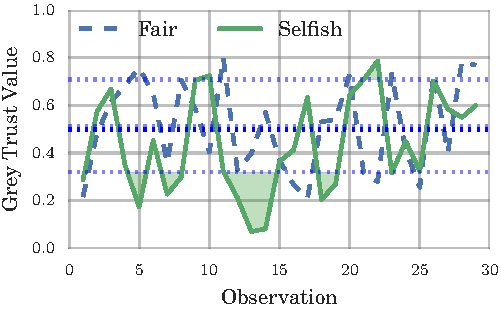
\includegraphics[width=\linewidth]{trust_bella_all_mobile_emph_ARXP_SelfishTargetSelection}
	\label{fig:all_mobile_selfish_rxp}
	\end{subfigure}
	\begin{subfigure}{0.45\textwidth}
	\caption{TX Power Emphasised}
	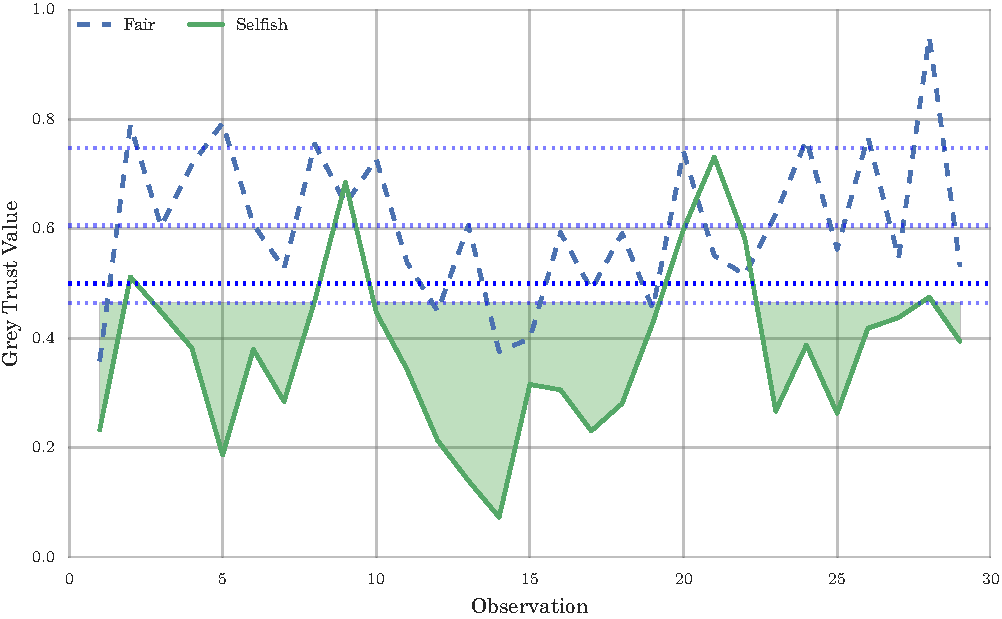
\includegraphics[width=\linewidth]{trust_bella_all_mobile_emph_ATXP_SelfishTargetSelection}
	\label{fig:all_mobile_selfish_txp}
	\end{subfigure}
	
	\begin{subfigure}{0.45\textwidth}
	\caption{RX Throughput Emphasised}
	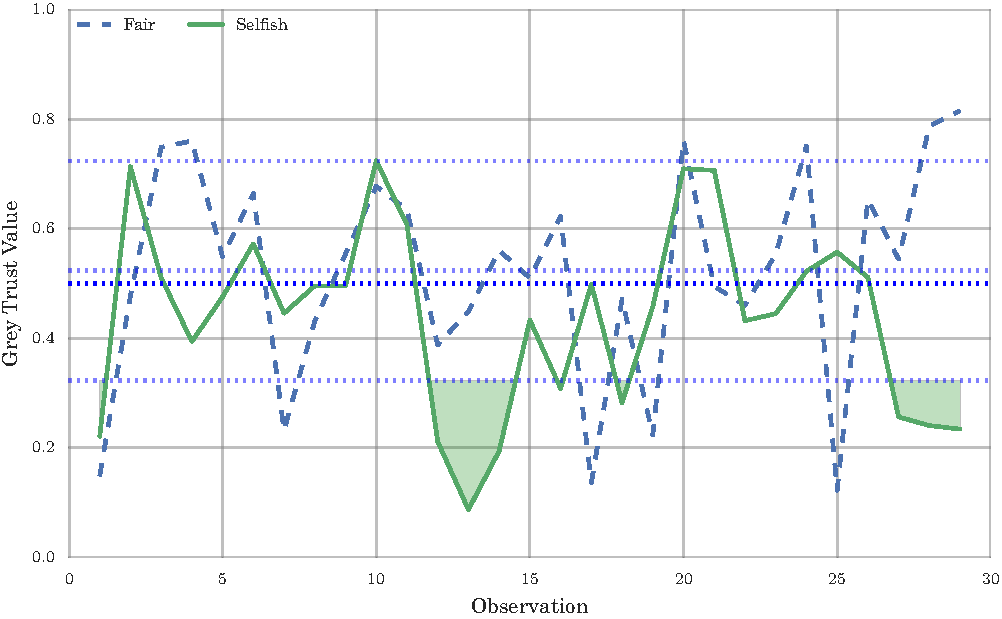
\includegraphics[width=\linewidth]{trust_bella_all_mobile_emph_RXThroughput_SelfishTargetSelection} 
	\label{fig:all_mobile_selfish_rxthroughput}
	\end{subfigure}
	\begin{subfigure}{0.45\textwidth}
	\caption{TX Throughput Emphasised}
	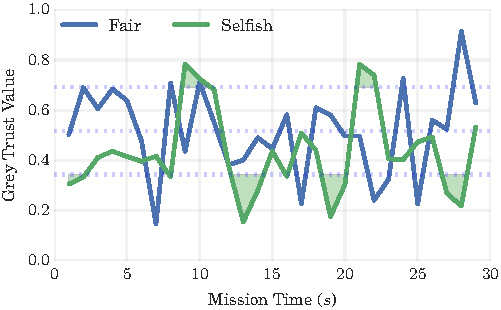
\includegraphics[width=\linewidth]{trust_bella_all_mobile_emph_TXThroughput_SelfishTargetSelection} \label{fig:all_mobile_selfish_txthroughput}
	\end{subfigure}
	\caption{$T_{1,MTFM}$ in the All Mobile case for the Selfish Target Selection behaviour, including dashed $\pm\sigma$ envelope about the fair scenario}
	\label{fig:all_mobile_selfish}
\end{figure}

From Fig.~\ref{fig:all_mobile_badmouthing} we can see that the malicious node is consistently outside the $\pm\sigma$ (one standard deviation above and below the mean) envelope of the fair scenario it's being compared to.
This is particularly true for PLR, with smaller impacts on delay, received power and transmitted throughput. 
This weighted delta in received throughput is minimal to insignificant compared to the width of the detection envelope, occasionally breaching the envelope for a short period. 

In the selfish case (Fig.~\ref{fig:all_mobile_selfish}) we observe much lower weighted delta in PLR and delay, with greatly increased impact on transmission power.
In comparison to \cite{Guo11}, these results are qualitatively similar, however here the differences between the fair case and the misbehaviours are less clear than in the comparable terrestrial space.
Guo et al. show similar types of behaviour but report a weighted delta from $\approx$ 0.4 to $\approx$ 0.9 across the simulation period, compared to our maximum delta in TX Power of $\approx$ 0.3 for an inconsistent interval (Fig.~\ref{fig:all_mobile_selfish_txp}.)


\subsection{Weight Significance Analysis for Behaviour Classification}

For a more quantitative assessment of the viability of multi-metric trust assessment methods, we take the qualitative analysis above and apply a Random Forest regression \cite{Breiman2001} to assess the relative importance of the selected metrics on relative detectability of malicious behaviour. 
Random Forest accomplishes this by generating a large number of random regression trees and prune these trees to fit incoming data.
The target function for this regression was the area between the target behaviours weighted $T_{MTFM}$ curve and the $\pm\sigma$ envelope of the base behaviour as shaded in Figs.~\ref{fig:all_mobile_badmouthing} and ~\ref{fig:all_mobile_selfish}.
From this training process we can extract the relative importance of each input feature (metric) in terms of how good it is to differentiate between the fair case and a given misbehaviour.
Additionally we perform a cross correlation analysis to establish the correlations between given metric weighting emphasis and the output of the target function.
Our intention is to establish the metrics that not only differentiate both misbehaviours from the fair case, but also what metrics differentiate the two misbehaviours from each other.

Applying this target regression to 729 different metric weight vector emphasis combinations reveals that each of the three combinations (i.e. comparing fair to misbehaviours, and comparing the misbehaviours) present distinct patterns of significance in three primary metrics; received throughput, transmitted power, and PLR, with delay, received power and transmitted throughput playing a lesser role.
Practically this means that in order to accurately distinguish between these scenarios, these primary metrics should be higher-weighted in the generation of $T_{1,MTFM}$ in \eqref{eq:networkeffects}.

It may initially appear odd that the relative significance of the received throughput is similar between all three scenario combinations, however a correlation analysis shows that in the MPC attack; the received throughput is positively correlated with successful classification against the fair case ($R=+0.71, p\approx10^{-100}$), while the inverse is the case for the STS attack ($R=-0.70, p\approx10^{-100}$).
It is expected that Transmitted power should be the defining characteristic of STS ($R=+0.72, p<10^{-100}$) as the node is acting fairly from a protocol perspective but is acting unfairly at a higher (incentive) level; it is performing fairly in terms of it's communications with other nodes, however it is preferring to communicate with nodes that it can expend less energy communicating with.
A summary of these correlations is shown in Table.~\ref{tab:correlations}.

Comparing Figs.~\ref{fig:otmf_beta_comparison},~\ref{fig:all_mobile_badmouthing_plr}, and ~\ref{fig:all_mobile_selfish_plr}, while it is possible that in a cleaner, less sparse, and less noisy environment, OTMF would be able to detect the MPC behaviour, from Fig.~\ref{fig:malselfactors} we see that PLR plays almost no part at all in detecting the STS behaviour, and so OTMF would not detect the attack.

\begin{figure}
	\centering
	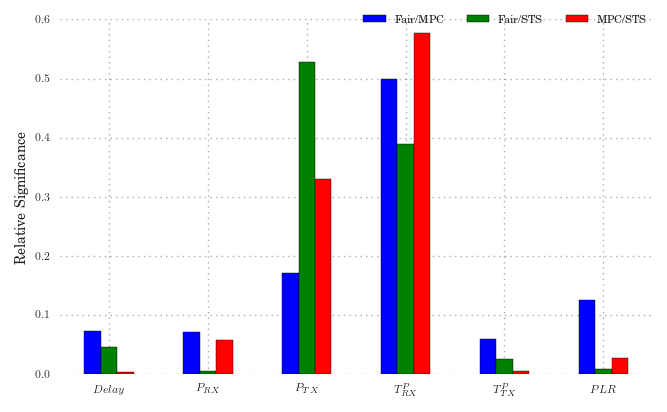
\includegraphics[width=0.95\linewidth]{MaliciousSelfishMetricFactors}
	\caption{Random Forest Factor Analysis of Malicious (MPC), Selfish (STS) and Fair behaviours compared against eachother}
	\label{fig:malselfactors}
\end{figure}

\begin{table}[h]
	\caption{Correlation Coefficients between metric weights and behaviour detection targets} \label{tab:correlations}
	\begin{center}
		\begin{tabular}{lcccccc}
			\toprule
			Correlation      & Delay & $P_{RX}$ & $P_{TX}$ & $T^P_{RX}$ & $T^P_{TX}$ & PLR \\
			\midrule
			Fair / MPC       & 0.199 &  0.159   & -0.416  &  0.708   & -0.238   & -0.401\\
			Fair / STS       & 0.179 &  -0.009  &  0.724  & -0.697   & -0.145   & -0.052\\
			MPC / STS        & 0.058 &  -0.134  &  0.146  & -0.768   &  0.052   &  0.146\\
			\bottomrule
		\end{tabular}
	\end{center}
\end{table}

As such this presents the open opportunity to develop a heuristic weight search scheme to detect malicious behaviour without the comparison to the fair scenario.
This would be accomplished by assessing the impact of differential metric weighting on the mean trust assessment rather than comparing co-weighted valuations across scenarios.


\section{Conclusions and Future Work}
We have demonstrated that existing MANET Trust Management Frameworks are not directly suitable to the sparse, noisy, and dynamic underwater medium.
We presented a comparison between trust establishment in MANETs in a simulated underwater environment, demonstrating that in order to have any reasonable expectation of performance, throughput and delay responses must be characterised before implementing trust in such environments. 
While the MTFM value does not display any immediate difference between the two behaviours, we have shown that by exploring the metric space by weight variation, the existence and nature of the malicious behaviour can be discovered.
Another difference is that MTFM is significantly more computationally intensive than the relatively simple Hermes / OTMF algorthms.
The repeated metric re-weighting required for real time behaviour detection is therefore an area that requires optimization.
We demonstrated initial, unfiltered Grey Trust assessment using all available metrics (transmitted and received throughput, delay, received signal strength, transmitted power, and packet loss rate), as well as the application of multiple weighting vectors to iteratively emphasise different aspects of trust operation to expose and identify misbehaviour on the network.
With significant delays (from seconds to many minutes), in a fading, refractive medium with varying propagation characteristics, the environment is not as predictable or performant as classical MANET TMF deployment environments.

We show that, without significant adaptation, single metric probabilistic estimation based TMFs are ineffective in such an environment.
We have shown that existing frameworks are overly optimistic about the nature and stability of the communications channel, and can overlook characteristics that are useful for assessing the behaviour of nodes in the network. 
This indicates that there is a good case, particularly within constrained MANETs as this, for multi-vector, and even multi-domain trust assessment, where metrics about the communications network and topology would be brought together with information about the physical behaviours and operations of nodes to assess trust.

Also, a significant factor of trust assessment in such a constrained environment, is that there may be long periods where two edge nodes (for instance, $n_0 \to n_5$) may not interact at all. 
This can be due to a range of factors beyond malicious behaviour, including simple random scheduling coincidence and intermediate or neighbouring nodes collectively causing long back-off or contention periods.
This disconnection hinders trust assessment in two ways; assessing nodes that do not receive timely recommendations may make decisions based on very old data, and malicious nodes have a long dwelling time where they can operate under a reasonable certainty that the TMF will not detect it (especially if the node itself is behaving disruptively).
One solution to this would be to move from a stepping-window of trust observations to a continuous trust log, updated on packet reception rather than waiting regular periods for packets to be analysed.
Future work will investigate the improvement of weight-based detection algorithms, the stability of GRA under multi-node collusion, the development of real-time outlier detection, and the introduction of physical behavioural metrics into the trust assessment context.



\subsection{Metric Weighting}
\begin{figure}
\begin{subfigure}{.5\textwidth}
  \centering
  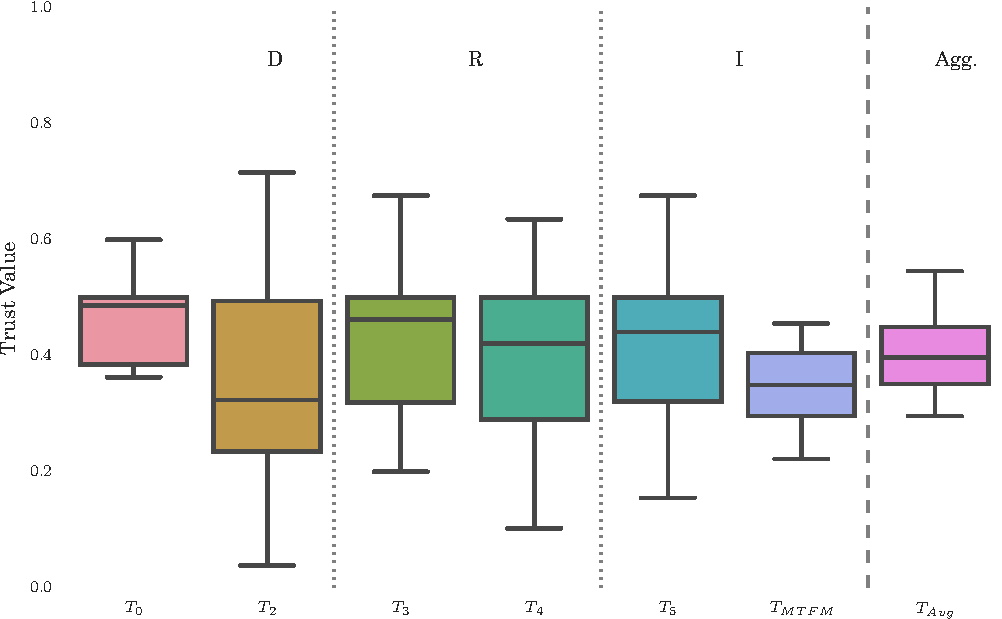
\includegraphics[width=.95\linewidth]{trust_bella_static_selfish.pdf}
  \caption{All Nodes Static}
  \label{fig:selfish_trust_static}
\end{subfigure}%
\begin{subfigure}{.5\textwidth}
  \centering
  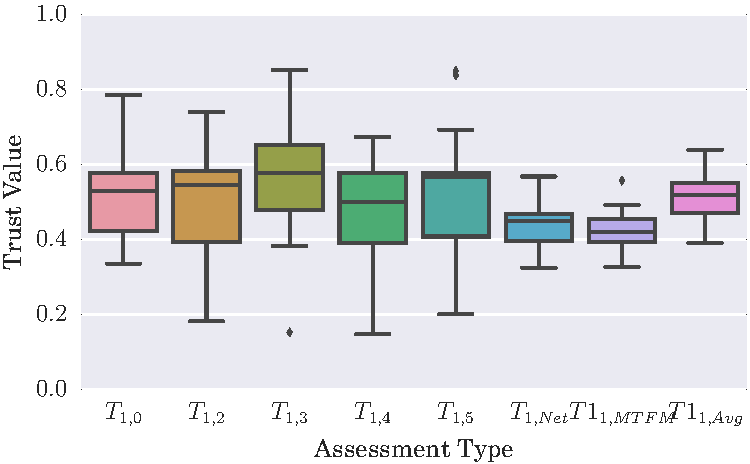
\includegraphics[width=.95\linewidth]{trust_bella_single_mobile_selfish.pdf}
  \caption{$n_1$ Randomly Walking}
  \label{fig:selfish_trust_single}
\end{subfigure}
\begin{subfigure}{.5\textwidth}
\centering
  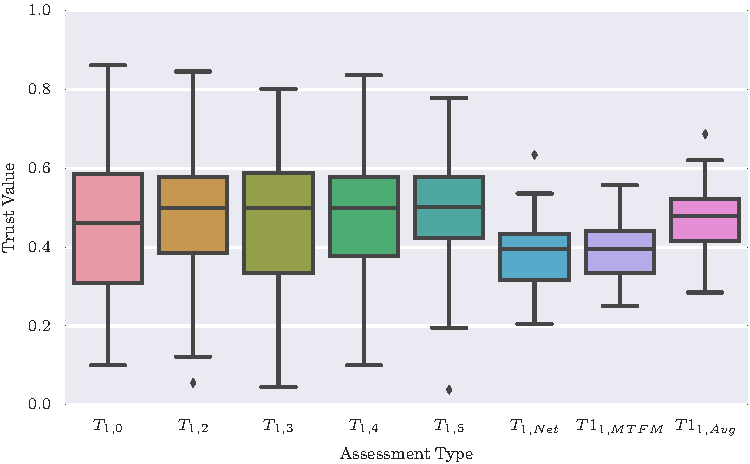
\includegraphics[width=.95\linewidth]{trust_bella_allbut1_mobile_selfish.pdf}
  \caption{All Nodes but $n_1$ Randomly Walking}
  \label{fig:selfish_trust_allbut1}
\end{subfigure}
\begin{subfigure}{.5\textwidth}
\centering
  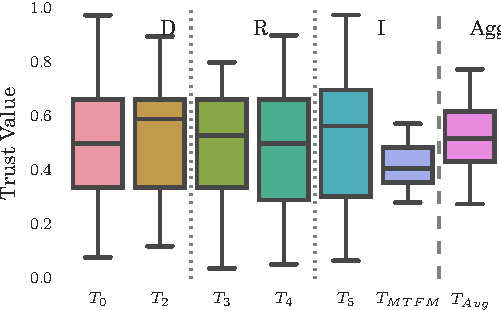
\includegraphics[width=.95\linewidth]{trust_bella_all_mobile_selfish.pdf}
  \caption{All Nodes Randomly Walking}
  \label{fig:selfish_trust_all_mobile}
\end{subfigure}
\caption{MTFM Trust assessments for varying mobility options in the selfish case}
\label{fig:trust_mobility}
\end{figure}



\begin{figure}
\begin{subfigure}{0.5\textwidth}
  \centering
  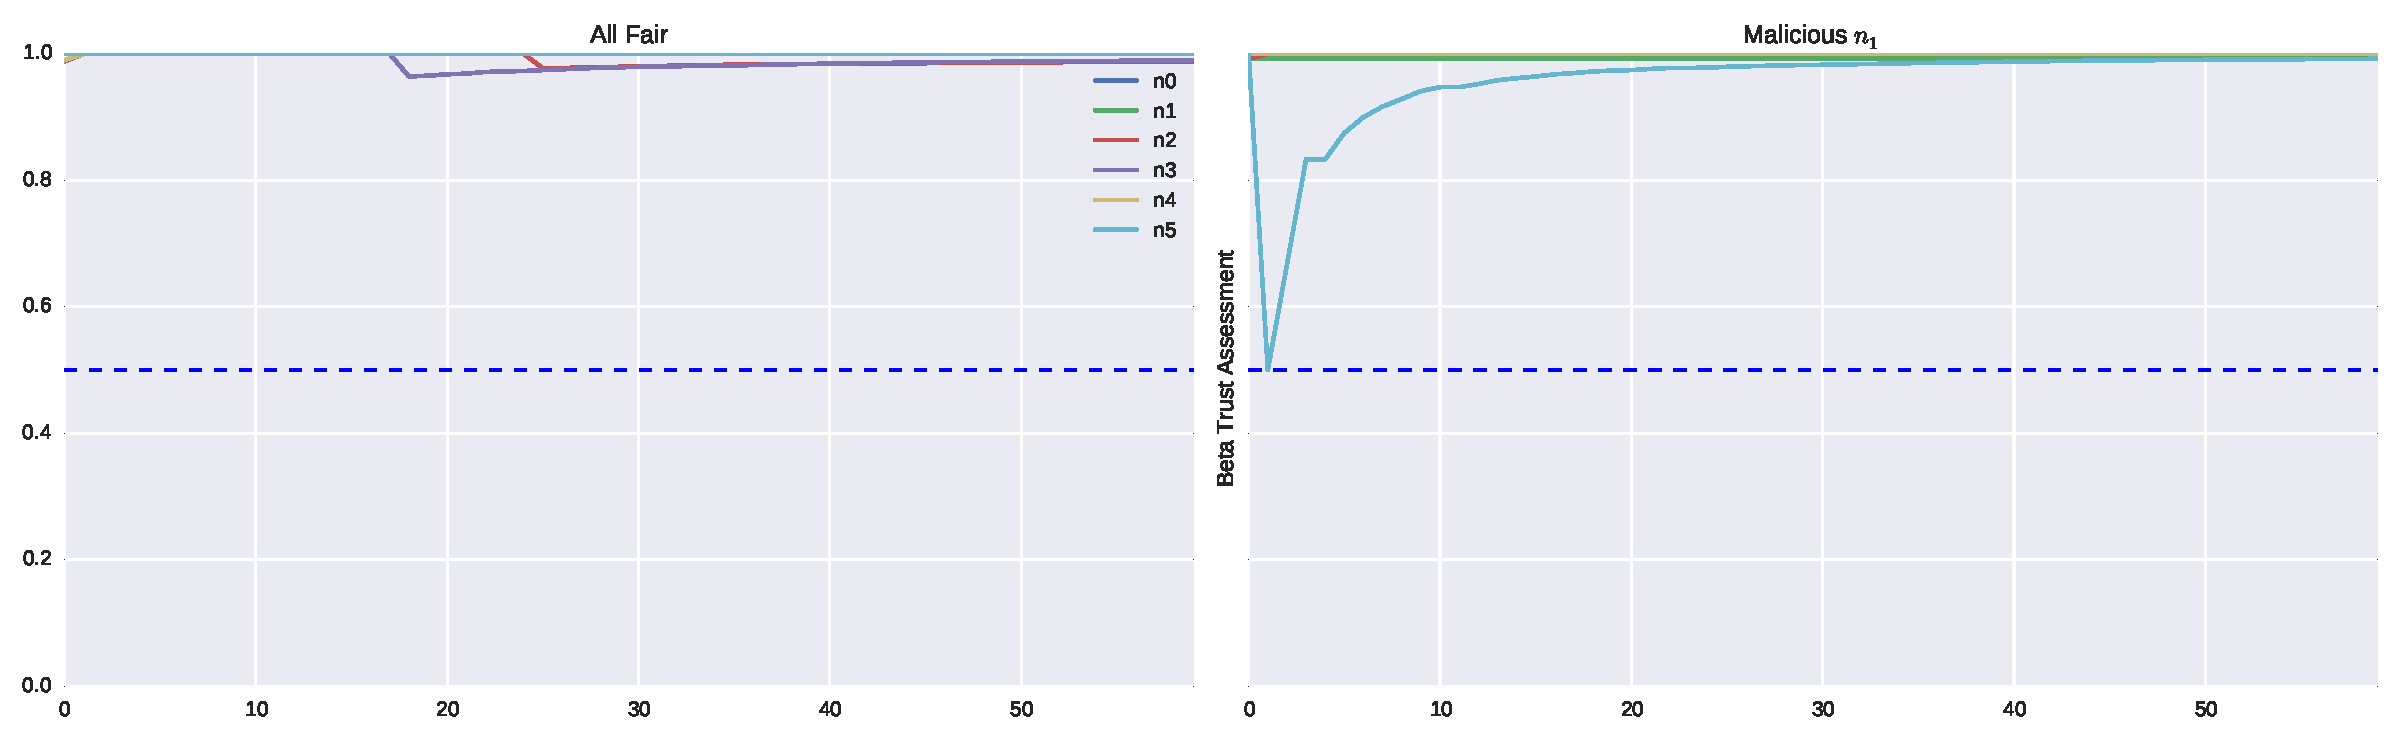
\includegraphics[width=.95\linewidth]{beta_trust_bella_static_joint.pdf}
  \caption{All Nodes Static}
  \label{fig:beta_trust_static}
\end{subfigure}%
\begin{subfigure}{0.5\textwidth}
  \centering
  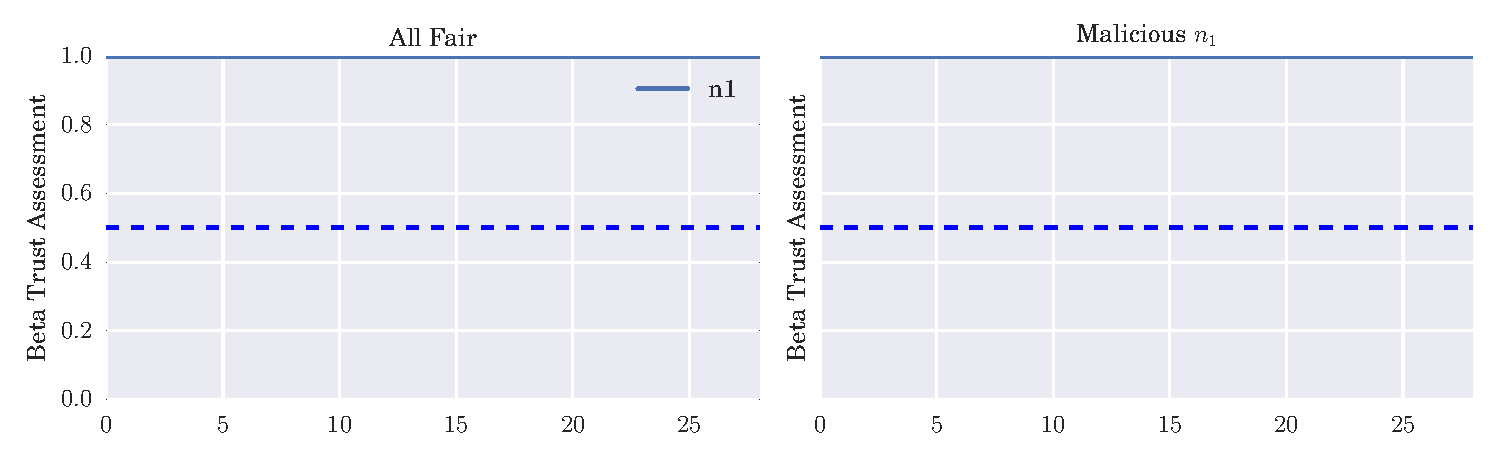
\includegraphics[width=.95\linewidth]{beta_trust_bella_single_mobile_joint.pdf}
  \caption{$n_1$ Randomly Walking}
  \label{fig:beta_trust_single}
\end{subfigure}%

\begin{subfigure}{0.5\textwidth}
\centering
  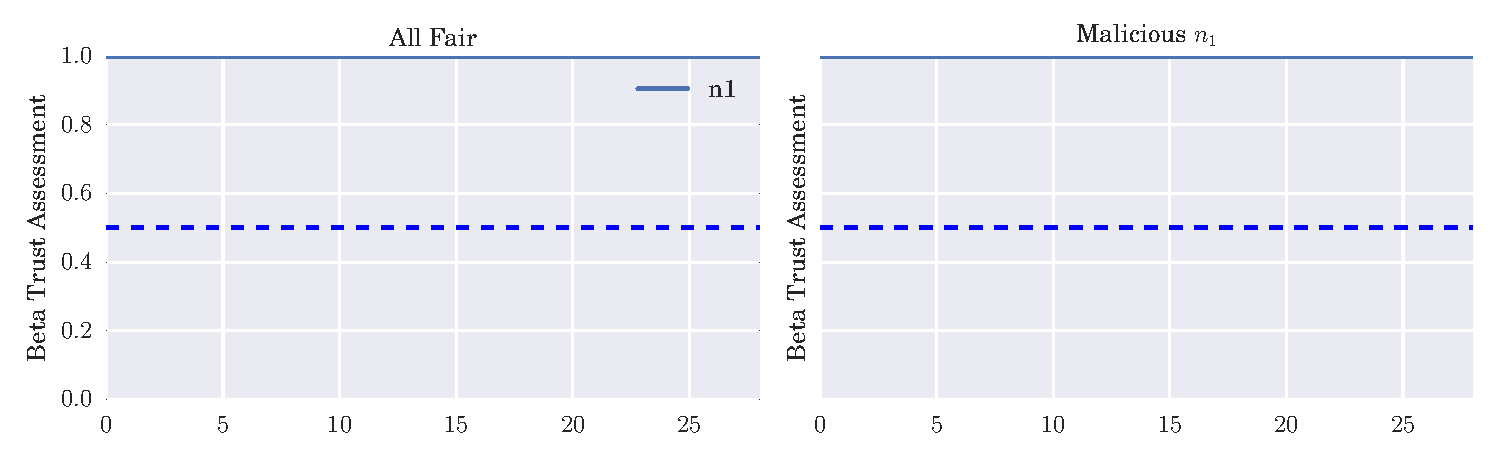
\includegraphics[width=.95\linewidth]{beta_trust_bella_allbut1_mobile_joint.pdf}
  \caption{All Nodes but $n_1$ Randomly Walking}
  \label{fig:beta_trust_allbut1}
\end{subfigure}%
\begin{subfigure}{0.5\textwidth}
\centering
  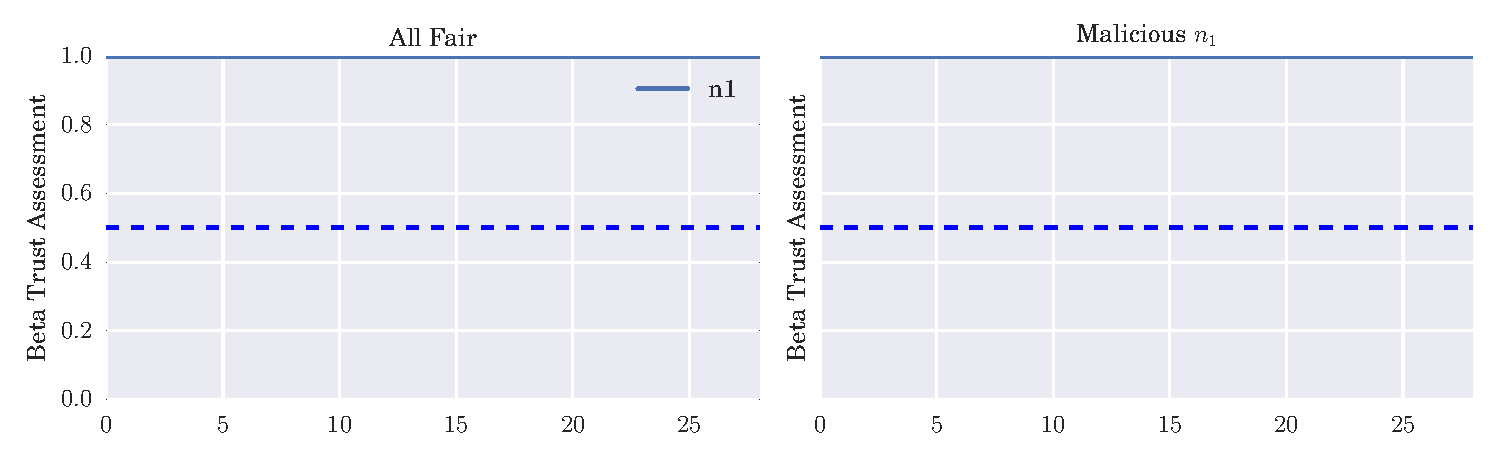
\includegraphics[width=.95\linewidth]{beta_trust_bella_all_mobile_joint.pdf}
  \caption{All Nodes Randomly Walking}
  \label{fig:beta_trust_all_mobile}
\end{subfigure}
\caption{Beta Trust time varying assessments for of $n1$ varying mobility options}
\label{fig:trust_mobility}
\end{figure}




%%%%%%%%%%%%%%%%%%%%%%%%%%%%%%%%%%%%%%%%%%%%%%%%%%%%%%%%%%%%%%%%%%%%%%%%%%%%%%%
\ifx\ifthesis\undefined
	%% ----------------------------------------------------------------
\label{Bibliography}
% \bibliographystyle{amsplain}
%\bibliographystyle{unsrtnat}  % Use the "unsrtnat" BibTeX style for formatting the Bibliography
\bibliographystyle{alpha}
\bibliography{../Thesis}  % The references (bibliography) information are stored in the file named "Thesis.bib"

\end{document}  % The End
%% ----------------------------------------------------------------
\else
\fi
